\documentclass{beamer}
\usetheme{metropolis}           % Use metropolis theme
\usepackage{textpos}
\usepackage[british,english,american]{babel}
\usepackage[british,english,american]{isodate}
\usepackage{bm}
\usepackage{amsmath}
\title{Development of a QMC code to tackle interacting electronic systems in 2D with application to TMD nanoribbons}
\selectlanguage{american}
\date{\printdate{2018-1-31}}
\author{Francisco Monteiro de Oliveira Brito}
\institute{
\includegraphics[scale = 0.2]{IST_A_CMYK_POS.eps} \hspace{40mm} 
\includegraphics[scale = 0.22]{fc_logo.png} \hspace{5mm} }

\begin{document}
  \maketitle
  \section{Beyond graphene: TMD nanoribbons}
  \begin{frame}{Graphene}
  	\metroset{block=fill}

	\begin{figure}
      \centering
      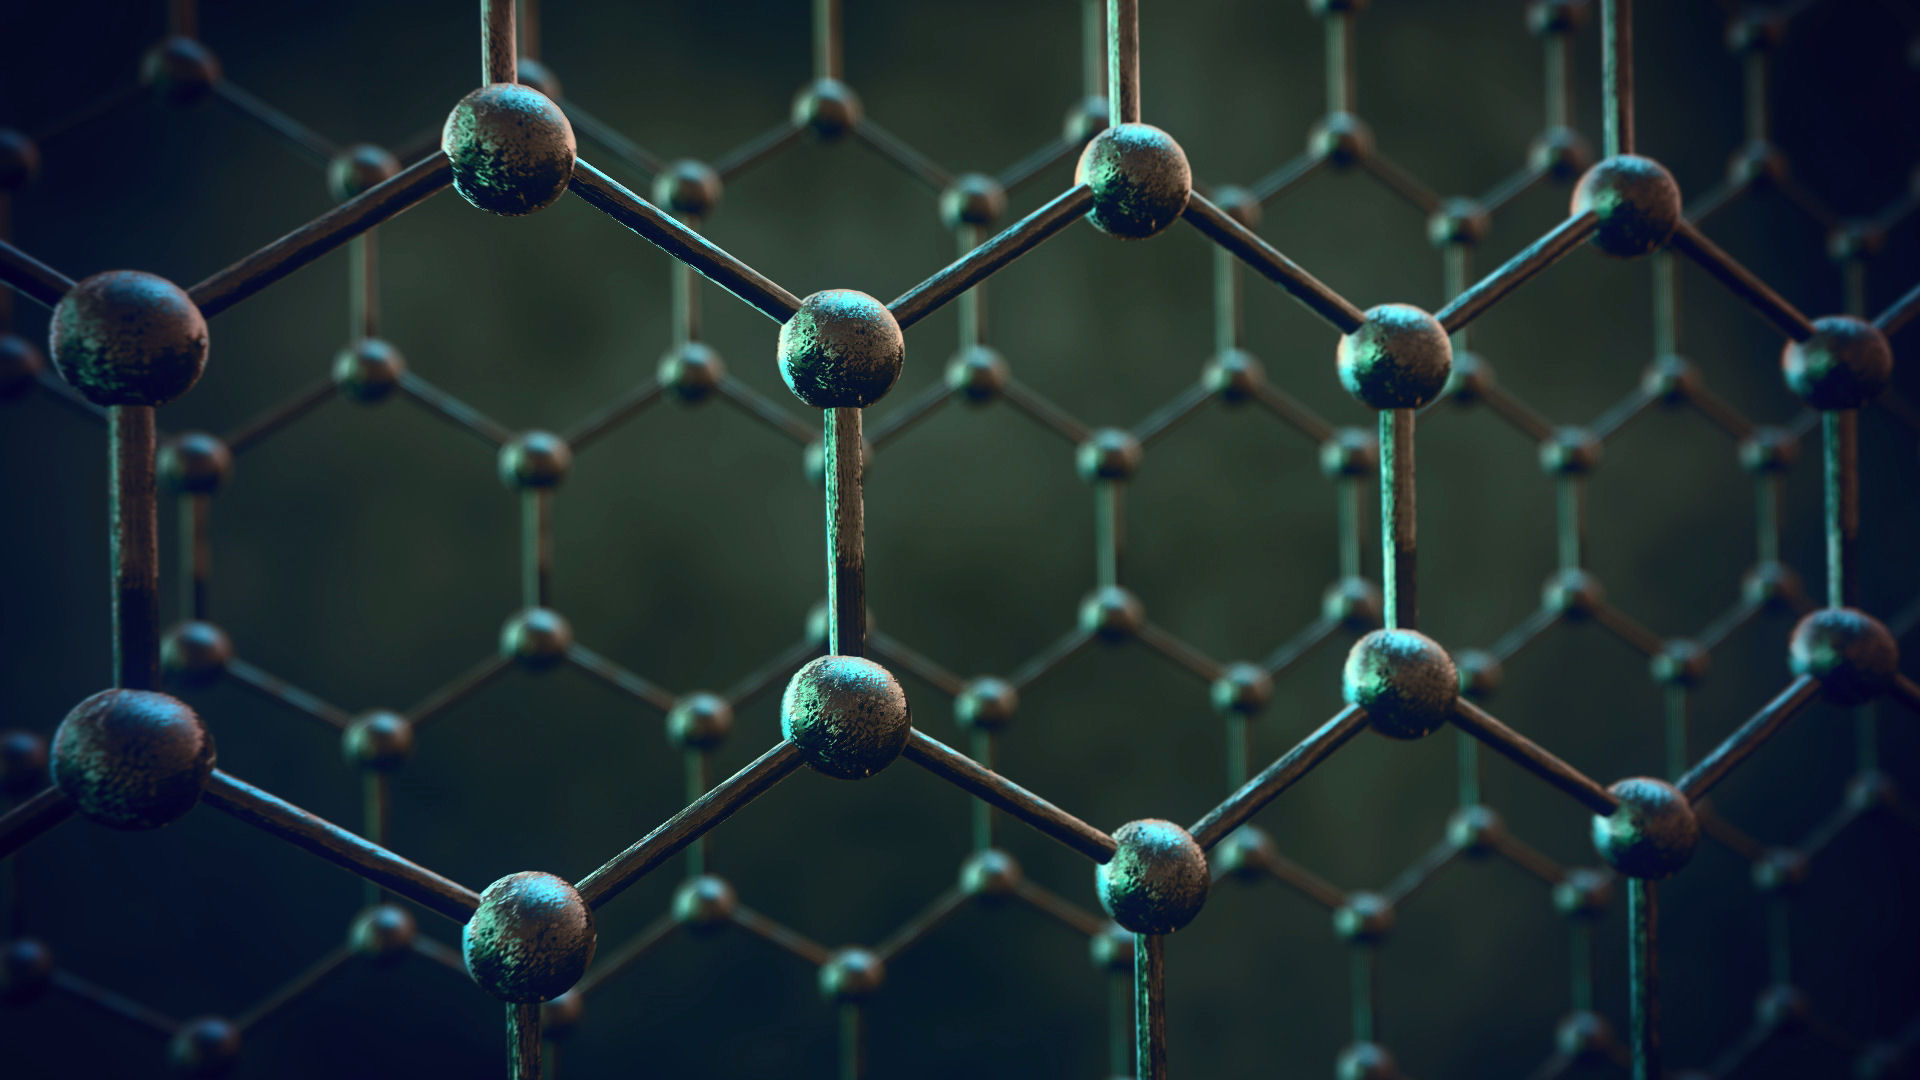
\includegraphics[scale = 0.06]{hexagonal-graphene-lattice-of-carbon-atoms.jpg}
 	 	\caption{Graphene's honeycomb lattice. (\href{http://www.graphene.manchester.ac.uk/}{graphene.manchester.ac.uk})}
      \end{figure}
      \begin{block}{Defying the Mermin Wagner Theorem}
        2D materials have been attracting interest since 2004, when graphene was isolated from a 3D graphite base (using scotch-tape), yielding a single layer of atoms.
      \end{block}

      \begin{block}{New perspectives}
        Graphene and graphene-like materials have promising properties, with interesting as-yet-unseen phenomena occurring within them.
      \end{block}
      
      
      
  \end{frame}
  
  \begin{frame}{Structure}
  \begin{figure}
  \centering
  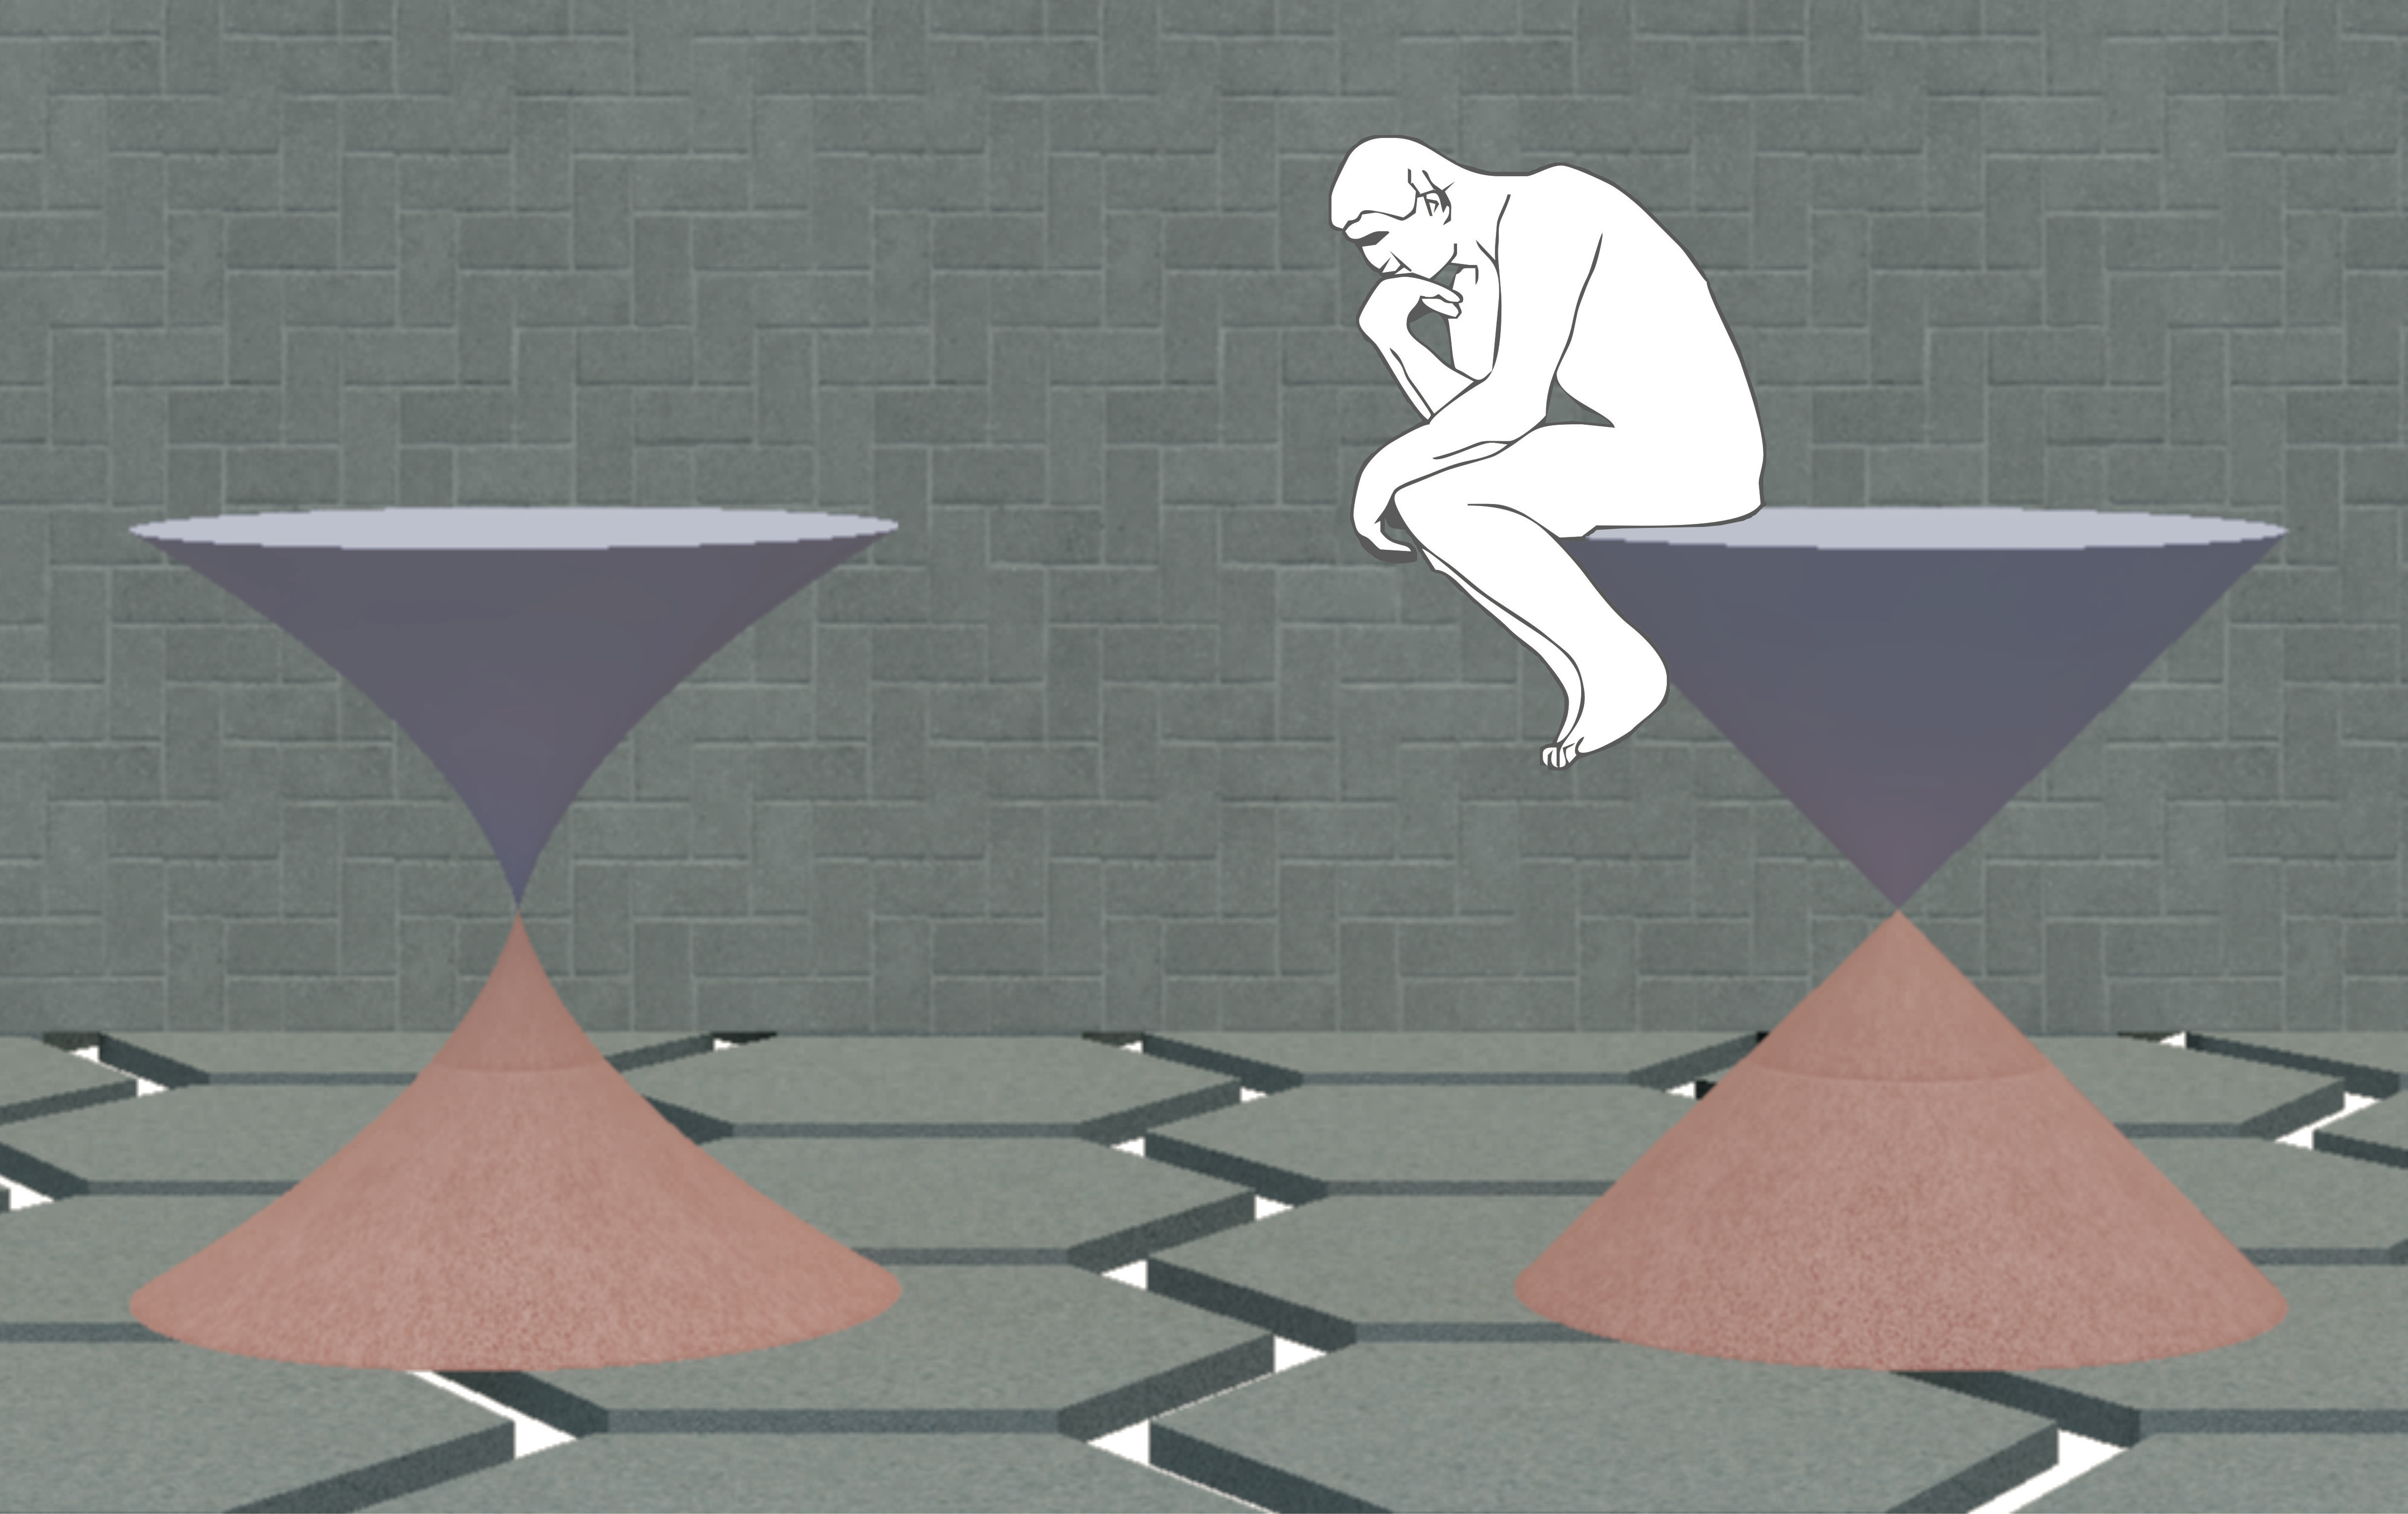
\includegraphics[scale = 0.028]{cones.jpg}
  \caption{Dirac cones. (from 
    \href{http://www.graphene.manchester.ac.uk/}{\emph{manchester}})}
   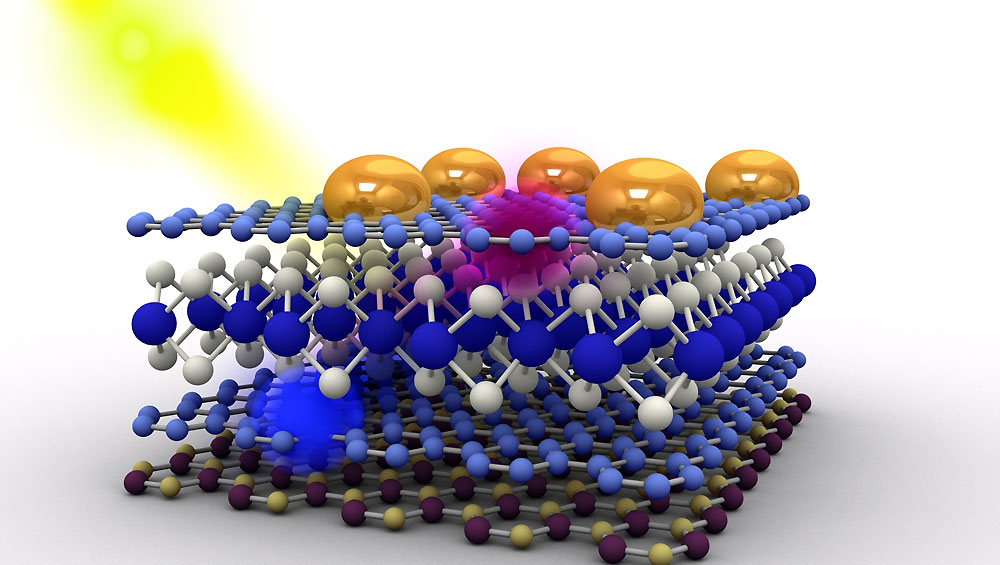
\includegraphics[scale = 0.135]{18-2D-atomic-crystals-image-library-01_1000x565.jpg}
  \caption{Heterostructure engineering. (from 
    \href{http://www.graphene.manchester.ac.uk/}{\emph{manchester}})}
   \end{figure}
  \end{frame}
  
  \begin{frame}{Interesting phenomena}
  \begin{figure}
  \centering
  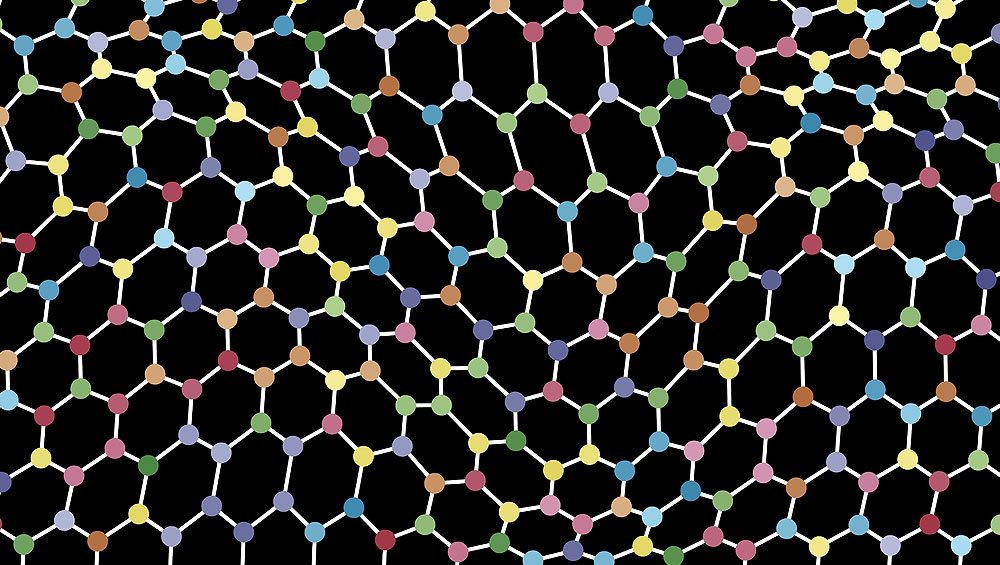
\includegraphics[scale = 0.143]{2-strain-in-graphene-image-library-01_1000x565.jpg}
  \caption{Strain creates pseudo magnetic fields. (from 
    \href{http://www.graphene.manchester.ac.uk/}{\emph{manchester}})}
   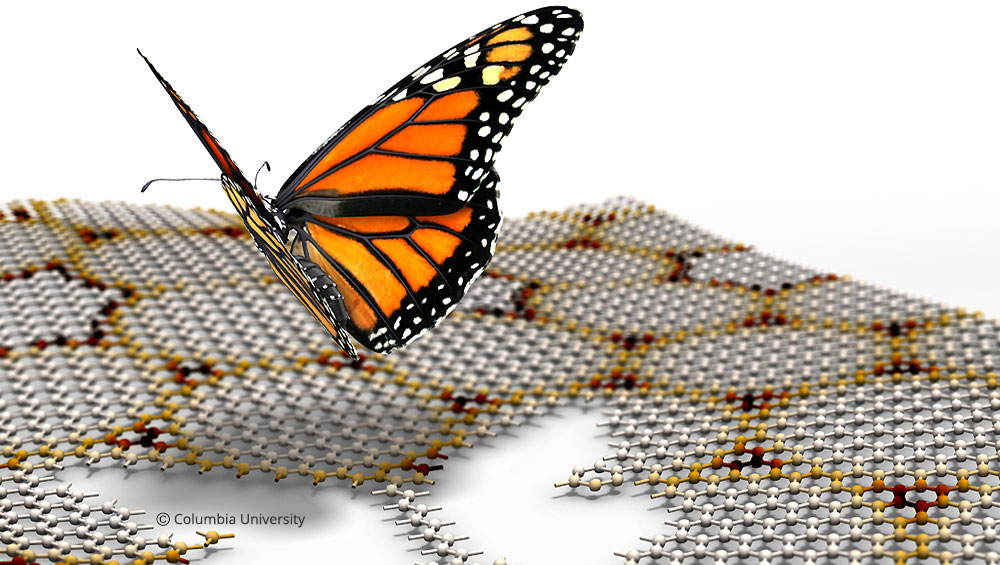
\includegraphics[scale = 0.145]{16-hofstadter-butterfly-image-library-01_1000x565.jpg}
  \caption{Hofstader's butterfly. (from 
    \href{http://www.graphene.manchester.ac.uk/}{\emph{manchester}})}
   \end{figure}
  \end{frame}
  
  \begin{frame}{Applications}
  \begin{figure}
  \centering
  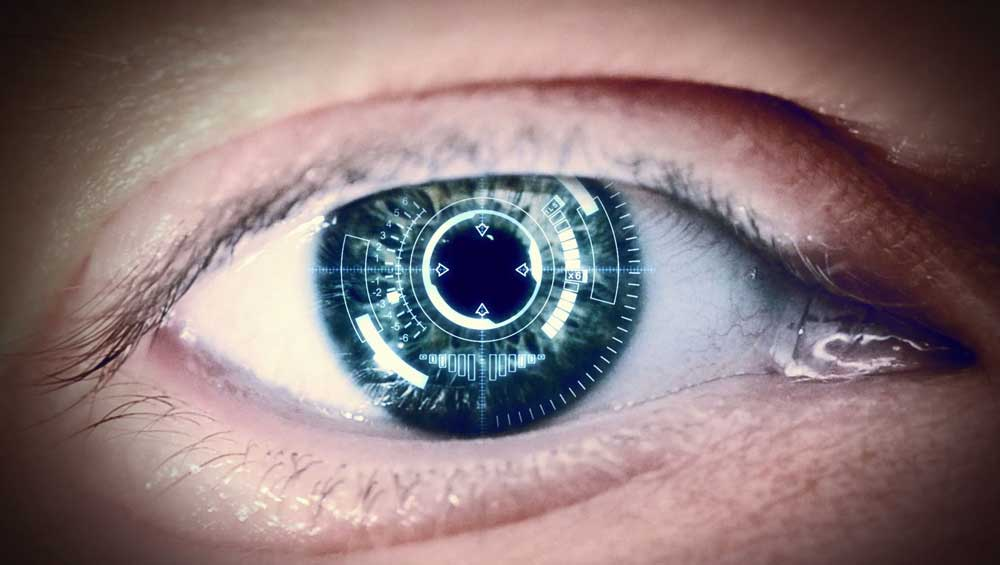
\includegraphics[scale = 0.138]{graphene-enhanced-contact-lense_1000x565.jpg}
  \caption{Smart contact lenses and night vision. (from 
    \href{http://www.graphene.manchester.ac.uk/}{\emph{manchester}})}
   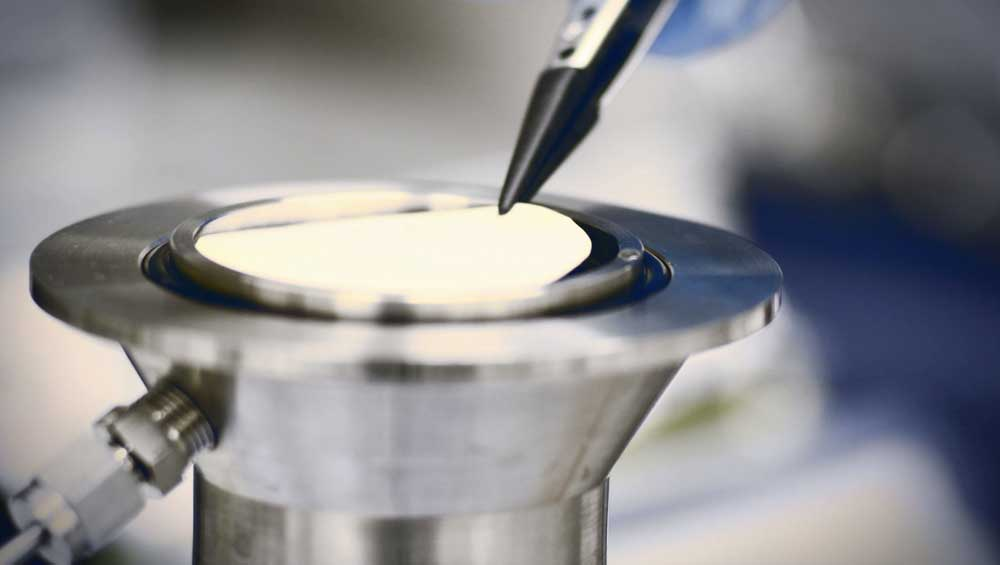
\includegraphics[scale = 0.14]{graphene-membrane_1000x565.jpg}
  \caption{Desalination and filtering of drinking water. (from 
    \href{http://www.graphene.manchester.ac.uk/}{\emph{manchester}})}
   \end{figure}
  \end{frame}
  
  \begin{frame}{Drawbacks}
  \metroset{block=fill}
  \begin{block}{Single layer graphene is gapless}
       ...while bilayer graphene has only a limited gap. A tunable gap is desirable in electronics applications.
      \end{block}

      \begin{block}{Superconductivity?}
       	A superconducting phase has been predicted for graphene. However, it is hard to achieve. It remains challenging to use it for applications.
      \end{block}
  \end{frame}  
  
  \begin{frame}{TMD nanoribbons: a possible solution}
  A nanoribbon consists of a 2D layer that is (nearly) infinitely long on one direction, but not on the other, so that edge states become relevant, and can be controlled to yield interesting properties.
  \metroset{block=fill}
  \begin{block}{Intrinsic gap $\rightarrow$ better switching}
        Advantageous to design electronic components.
      \end{block}

      \begin{block}{Topological superconductivity}
        \textit{Electron interactions} could be responsible for the appearance of a promising superconducting phase.
      \end{block}
      
      \begin{figure}
  \centering
  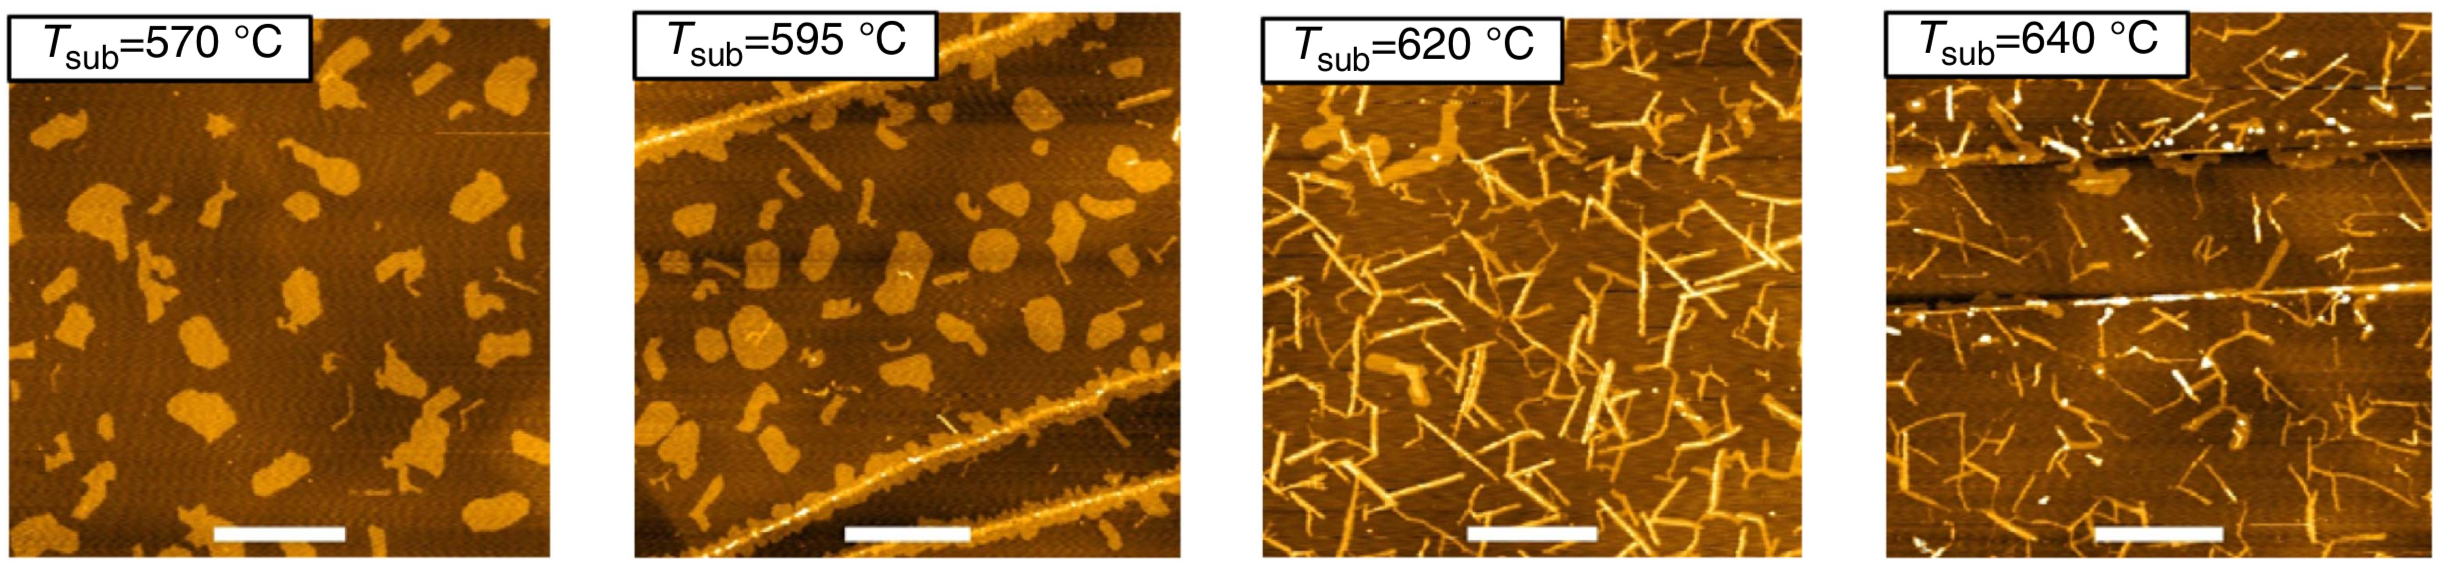
\includegraphics[scale = 0.2]{nanoribbons}
  \caption{Fabrication of TMD nanoribbons. (from 
    \href{https://www.nature.com/articles/ncomms15135}{\emph{Chen et al. 2017}})}
   \end{figure}
      
  \end{frame}    
  
	\begin{frame}{$e^- - e^-$ interactions and magnetism of metallic zigzag edges}
	\vspace{2mm}
	\metroset{block=fill}
	\begin{block}{Origin of magnetism}
       	A high density of low-energy electronic states is localized at the zigzag edges, decaying quickly in the bulk, which suggests the possibility of magnetic ordering.\\ \textbf{MF Hubbard} $\rightarrow$ magnetic moments localized at the edges.
      \end{block}	
	
	\begin{figure}[ht!]
	\hspace{-3.5cm}
\begin{minipage}[c]{0.1\textwidth}
\centering
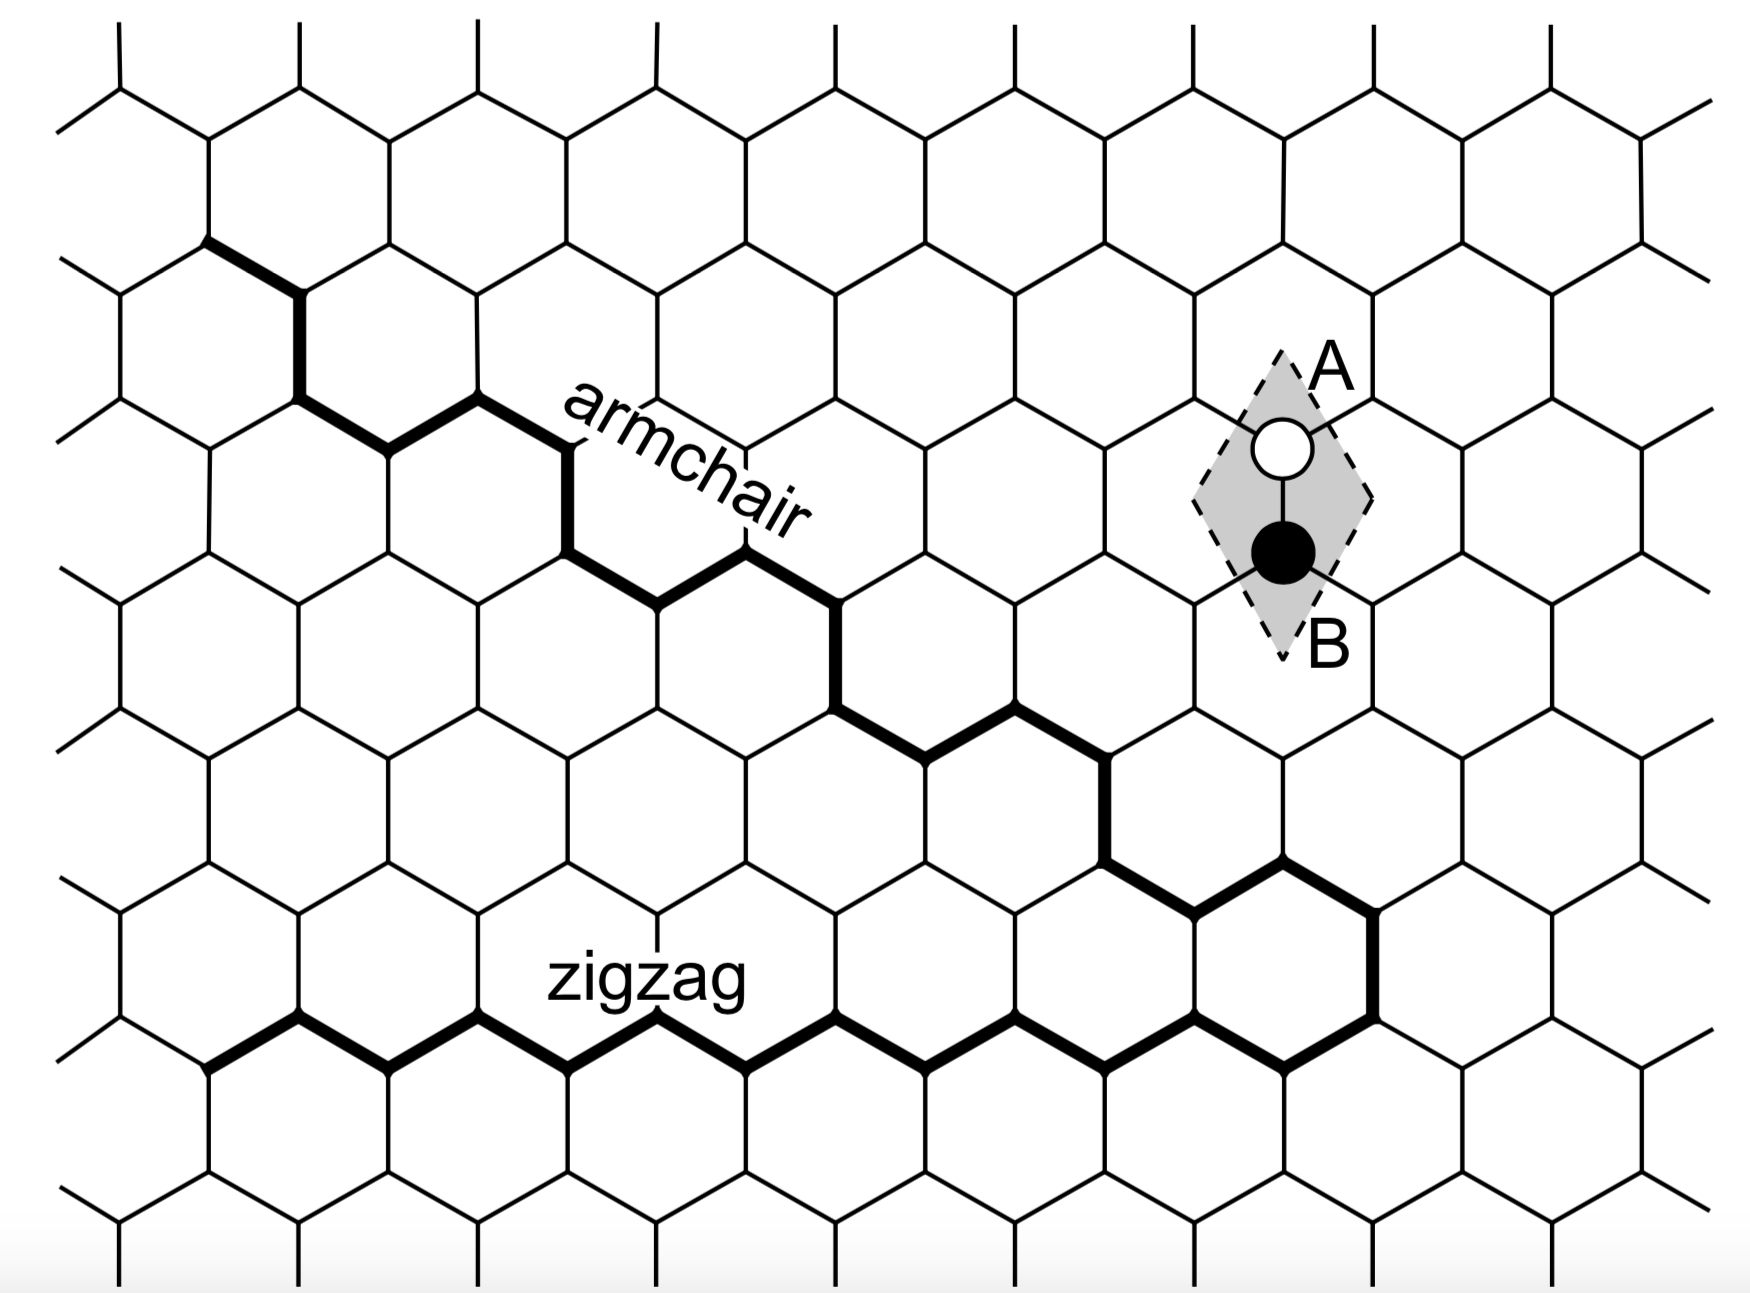
\includegraphics[scale = 0.142]{zigzag}
\end{minipage} \hspace{4cm}
\begin{minipage}[c]{0.1\textwidth}
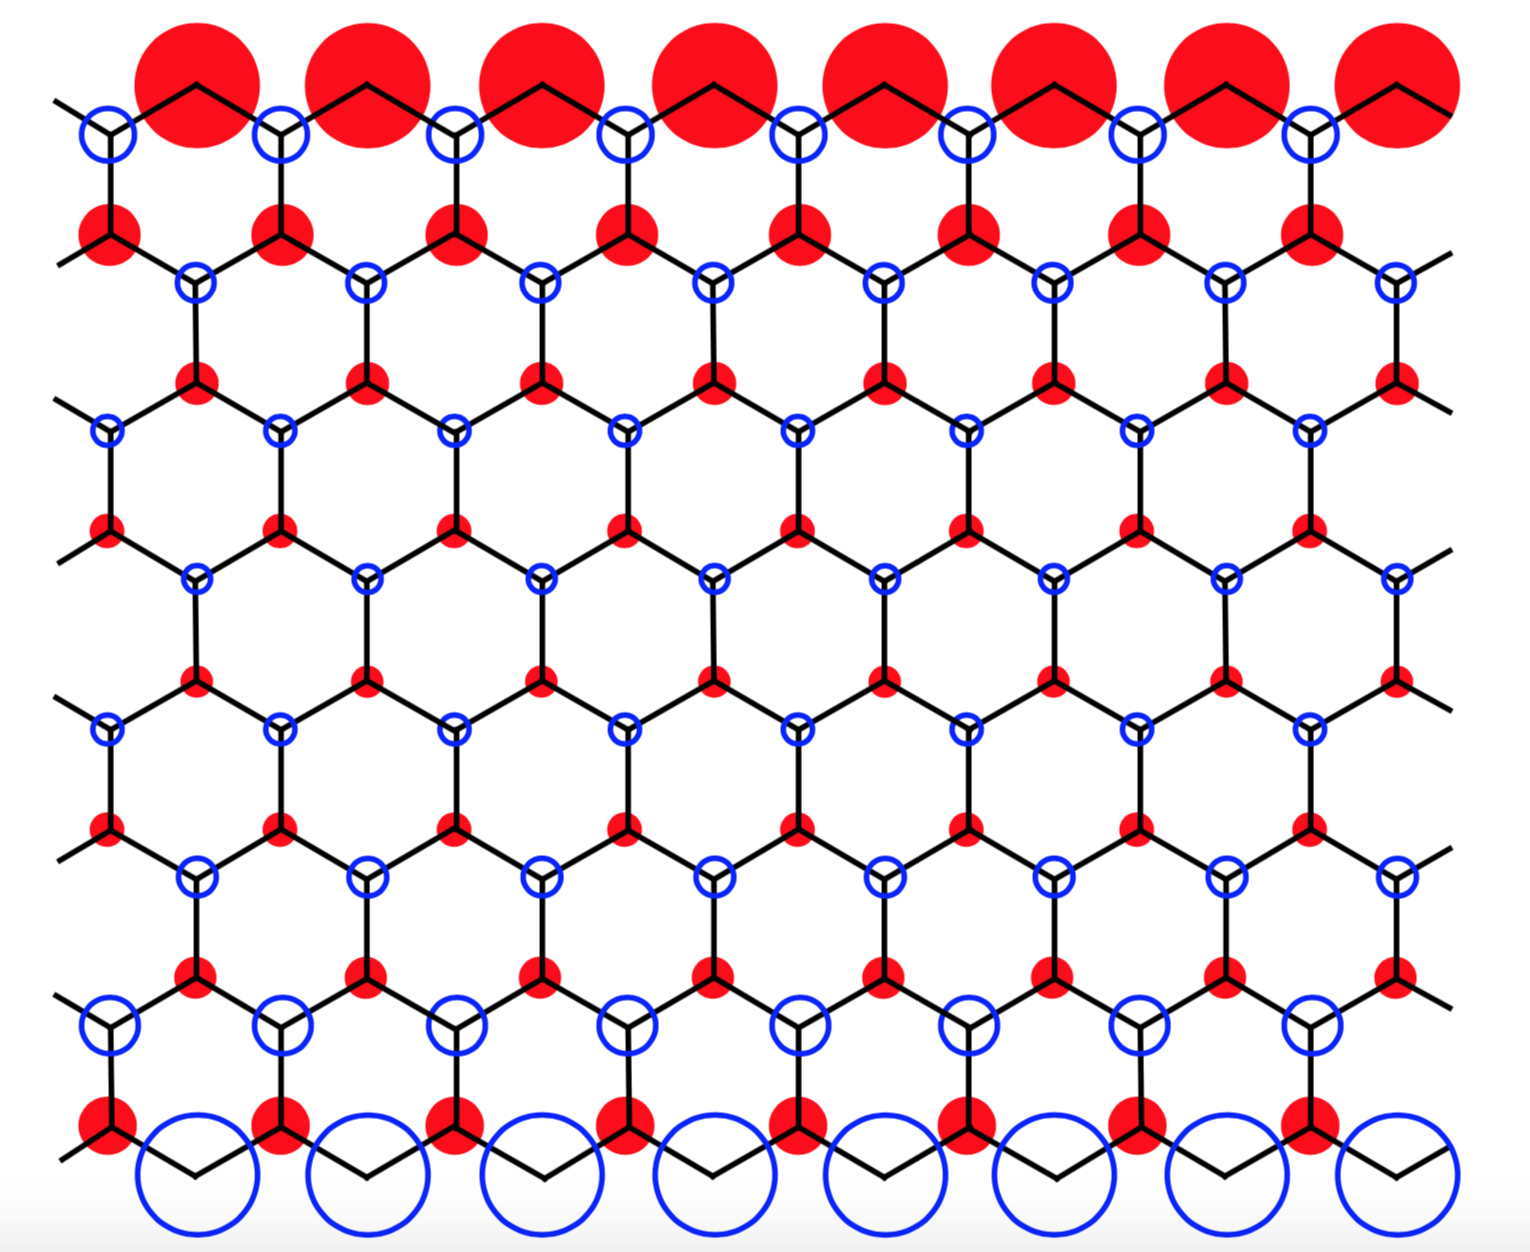
\includegraphics[scale = 0.148]{edge_states}
\end{minipage}
 \caption{Left: 2 possible edges of a nanoribbon in a honeycomb lattice. Right: Accumulation of $e^-$ edge states, corresponding to an AF ground state (opposite edges with opposite spins). (from 
    \href{https://arxiv.org/pdf/1004.2034.pdf}{\emph{Yazyev 2010}})}
\end{figure}

\end{frame}

\begin{frame}{Magnetic ordering of zigzag edges}

While the zigzag graphene nanoribbon antiferromagnetic ground state is semiconducting, a state with interedge ferromagnetic orientation is a metal. An example of an application based on the switching between the two states is a magnetorresistive sensor.

	\begin{figure}[ht!]
	\hspace{-3cm}
\begin{minipage}[c]{0.1\textwidth}
\centering
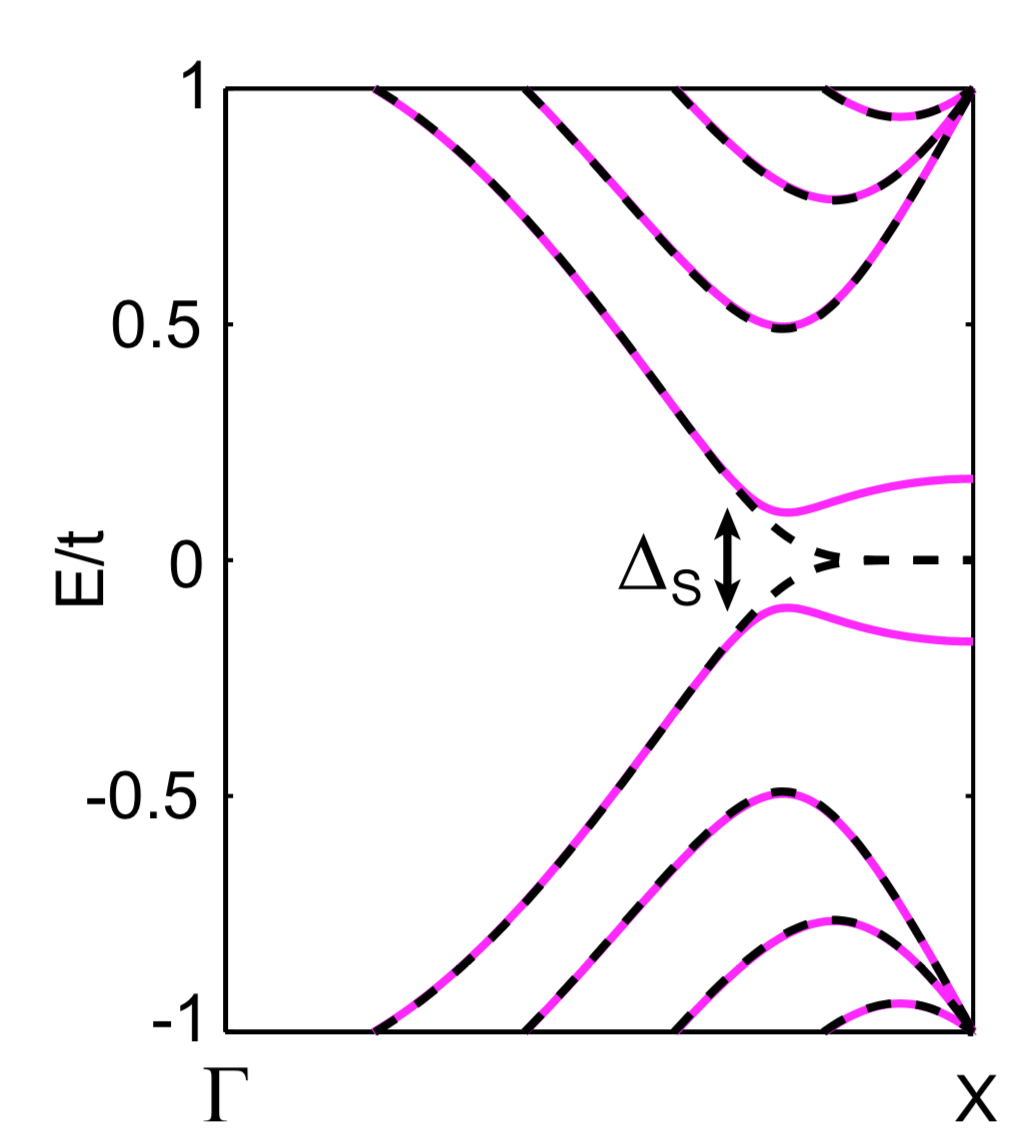
\includegraphics[scale = 0.177]{AF_GS}
\end{minipage} \hspace{4cm}
\begin{minipage}[c]{0.1\textwidth}
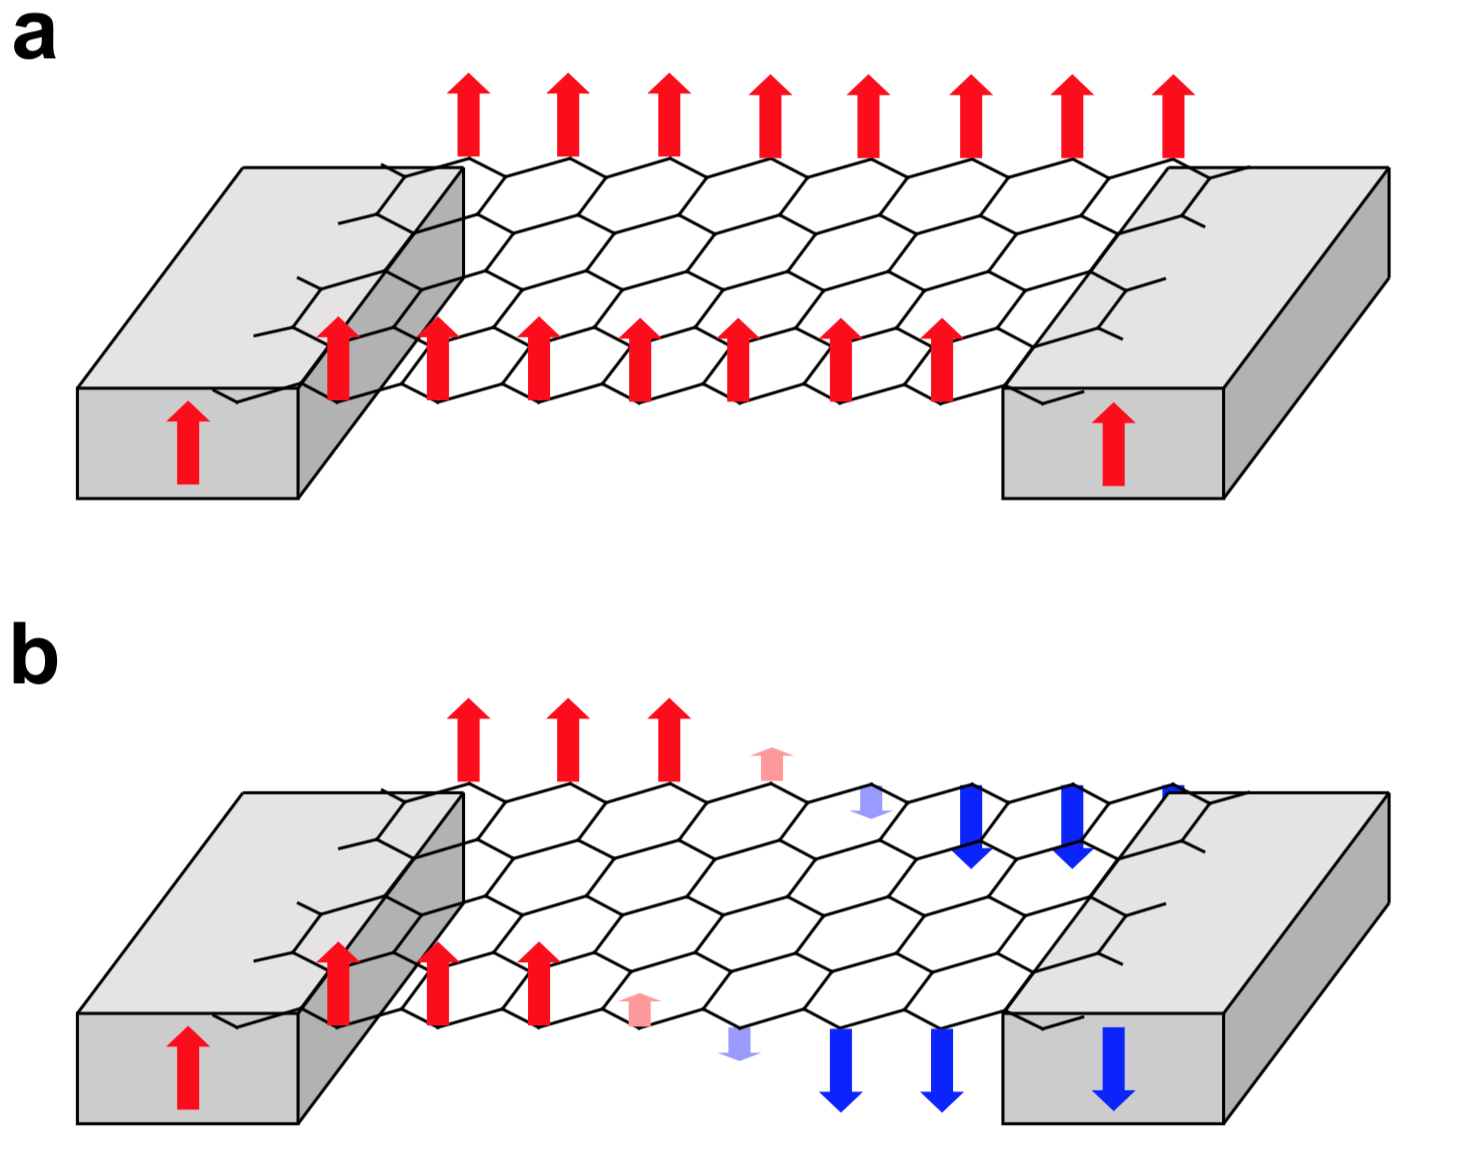
\includegraphics[scale = 0.157]{magnetoresistance}
\end{minipage}
 \caption{Left: Opening of a gap $\Delta_S$ due to electron interactions, for $U/t = 1.2$. Right: Switching between low (a) and high-resistance (b) configurations, corresponding, respectively, to parallel, and antiparallel configurations of the ferromagnetic leads. (from 
    \href{https://arxiv.org/pdf/1004.2034.pdf}{\emph{Yazyev 2010}})}
\end{figure}

\end{frame}
  
  \section{Monte Carlo}
 	 
  \begin{frame}{Exploiting randomness}

	\begin{figure}
 	 \centering
      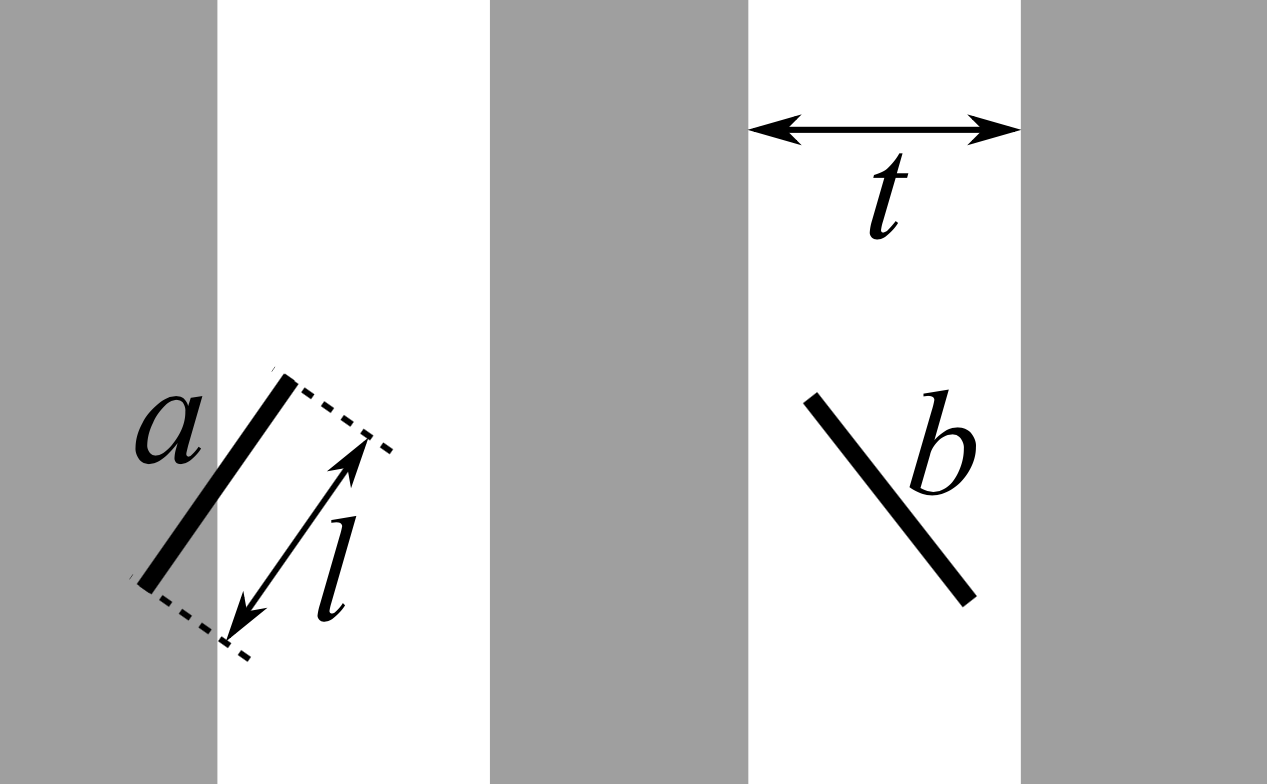
\includegraphics[scale = 0.18]{buffon}
 	 \caption{Buffon's experiment.}
 	 \end{figure}  
  
  	\metroset{block=fill}
  \begin{block}{Buffon (1777)}
        Estimate $\pi$ by repeatedly throwing a needle onto a sheet of paper with evenly spaced lines. $\pi = \lim_{N\rightarrow \infty} \frac{2Nl}{Mt}$
      \end{block}

      \begin{block}{Metropolis (1949)}
        More generally, we may produce accurate estimates of deterministic  integrals by using randomness.
      \end{block}
      
  \end{frame}
  
  \begin{frame}{Classical Monte Carlo}
  
	\begin{itemize}
	\item Integral as \textbf{expectation} of a random variable.
	\item Draw independent samples: a good \textbf{approximation} of the integral is the \textbf{sample mean}.
	\item To do this, design an \emph{ergodic} \textbf{Markov Chain} with a stationary distribution coinciding with the desired one.
	\item After the \emph{warm up} steps, the algorithm generates samples from the target distribution.
	\item Perform \textbf{independent measurements} of physical quantities (introducing decorrelation steps between them).
	\end{itemize}  
  
  \end{frame}
  
  \begin{frame}{Classical Monte Carlo}
  
  \metroset{block=fill}
  \begin{block}{Detailed balance}
        Let $\mu$ and $\nu$ be two possible states of the system. On average, transitions between $\mu$ and $\nu$ are just as frequent as those from $\nu$ to $\mu$. This corresponds to time-reversal symmetry, related to the concept of reversibility in thermodynamics.
      \end{block}

      \begin{block}{Importance sampling}
        Drastically improves convergence speed. This is done by variance reduction. An acceptance-rejection scheme is implemented to ensure that we focus on the most representative part of the state space.
      \end{block}

  \end{frame}
  
	\begin{frame}{Classical Monte Carlo}

	Suppose you want to measure the average of a given \emph{classical} quantity $Q$.  
  
	\begin{equation*}
	\left\langle Q \right \rangle = \frac{\sum_\mu Q_\mu e^{-\beta E_\mu}}{\sum_\mu e^{-\beta E_\mu}}
	\end{equation*}
	
	Very expensive because it requires the computation of the energies of all possible configurations.
	
	Solution: \textbf{Choose only a subset of states} at random with probability (distribution) $p_\mu$.

  \end{frame}  
  
  	\begin{frame}{Classical Monte Carlo}

	The estimator of the expectation becomes
	
	\begin{equation*}
	Q_{MC} = \frac{\sum_{i=1}^M Q_{\mu_i} p_{\mu_i}^{-1} e^{-\beta E_{\mu_i}}}{\sum_{j=1}^M p_{\mu_j}^{-1} e^{-\beta E_{\mu_j}}} 
	\end{equation*}

  \end{frame}  
  
    \begin{frame}{Classical Monte Carlo}
  
  	Approximate by drawing $M$ samples, and taking the sample mean.
  	
  	\textbf{Na\"ive estimator} ($p_\mu \sim$ Uniform distribution)
  		\begin{equation*}
    		Q_U = \frac{\sum_{i=1}^M Q_{\mu_i} e^{-\beta E_{\mu_i}}}{\sum_{j=1}^M e^{-\beta E_{\mu_j}}} 
 		\end{equation*}

      \textbf{Importance sampling} ($p_\mu \sim$ Boltzmann distribution)
      	\begin{equation*}
    		Q_B = \frac{1}{M} \sum_{i=1}^M Q_{\mu_i}
 		\end{equation*}

  \end{frame}
  
  \begin{frame}{So what?}
  
	\metroset{block=fill}
  	\begin{block}{Quantum Monte Carlo}
        Instead of simulating thermal fluctuations, we use analogous techniques to simulate \emph{quantum} fluctuations.
     \end{block}  

  \end{frame}
  
  \section{Variational Monte Carlo}
  	\begin{frame}{Variational principle}
	  	\metroset{block=fill}
	  	\begin{block}{Give your best guess}
  	We introduce a trial wave function $\phi (\bm r)$ with adjustable parameters $\bm \alpha$. 
  		\end{block}
  		\begin{block}{Optimize it}
  	The expectation we wish to approximate may be written as an integral, i.e. we optimize according to equation (\ref{eq:vmc}).
  	\end{block}
  	\begin{equation}\label{eq:vmc}
    E (\{\alpha_i \}) = \frac{\left\langle \phi | \mathcal{H} | \phi \right\rangle}{\left\langle \phi | \phi \right\rangle} = \frac{\int \phi^\star (\bm r) \mathcal{H} \phi (\bm r) d\bm r}{\int | \phi (\bm r') |^2 d\bm r'} \ge E_0
  	\end{equation}
  	
  	\end{frame}
  \section{Diffusion Monte Carlo}
  \begin{frame}{Schr\"odinger equation in imaginary time $\tau = -it$}
  \metroset{block=fill}
  \begin{block}{What if we cannot come up with a good guess?}
  	A reliable trial wave function may be difficult to construct. The many-body system can be simulated with less \emph{a priori} knowledge of its properties.
  	\end{block}
  	
  	 A Wick rotation turns the Schr\"odinger equation into the diffusion equation. Additionally, shifting the energy scale,
  	
  	\begin{equation*}
  	\partial_\tau \psi = -\frac{1}{2m} \partial_x^2 \psi -  \bigg[ V(x) - E_T \bigg] \psi
  	\end{equation*}
  \end{frame}
  
  \begin{frame}{Ground state as the last man standing}
  
  \metroset{block=fill}
  \begin{block}{Transient family}
  	The mapping $\tau = -it$ allows us to recast the eigenfunctions of the hamiltonian as a family of transients $e^{-E_n \tau}$.
  	\end{block}
  	\begin{block}{The last survivor}
  	 In the new time, the longest lasting transient corresponds to the ground state. 
  	 \end{block}
  	 
  	 Thus, for any $\psi (x, \tau)$ with which we start the algorithm:
  	
  	\begin{equation*}
  	\lim_{\tau \rightarrow \infty} \psi (x, \tau) \propto \phi_0 (x)
  	\end{equation*}
  \end{frame}
  
%  \begin{frame}{Generate samples using the \emph{exact} ground state wave function}
%  	The ground state energy may be written as an average \emph{local energy} over a distribution, which we compute using Monte Carlo.
%  	
%  	\begin{equation*}
%  	E_0 = \frac{ \left\langle \phi_0 | \mathcal{H} | \phi \right\rangle}{\left\langle \phi_0 | \phi \right\rangle} = \frac{\int d\bm r \phi_0^\star (\bm r) \phi (\bm r) E_L (\bm r)}{\int d\bm r\phi_0^\star (\bm r) \phi (\bm r)}
%  	\end{equation*}
%  	\end{frame}
%  \section{Path integral formulation}
%  \begin{frame}{Imaginary time evolution}
%
%  	The problem may be reformulated so as to eliminate errors due to the finite time step.
%  	
%  	\begin{equation*}
%  	\psi (\bm r_f, t)  = \int d\bm r_i G ( \bm r_f | \bm r_i ; \tau ) \psi (\bm r_i) ,
%  	\end{equation*}
%  	where the Green function, the imaginary-time propagator, is the matrix element $ G ( \bm r_f | \bm r_i ; \tau ) = < \bm r_f | e^{-(\mathcal{H} - E_T )\tau} | \bm r_i >$. This results in a path integral formulation of the random walk in configuration space.
%  \end{frame}
  \section{The sign problem for many-fermion systems}
  \begin{frame}{Fixed-Node approximation}
  \metroset{block=fill}
  
  \begin{block}{Many-fermion systems are tricky to simulate}
  	The \textit{antisymmetric} many-fermion wave function causes a numerical instability, associated with its \textbf{nodes}.
	\end{block}
	\begin{block}{Circumventing the problem}
  	Force convergence to the fermionic wave function by \textbf{fixing the nodes of the trial wave function} as the same as those of the fermionic ground state.
	\end{block}  	
	\begin{block}{In a nutshell}
	Diffusion method applied to $\mathcal{H}_{FN}$, which is simply the model hamiltonian with infinite potential barriers at the nodes of $\psi (\bm r)$  	 
  	 \end{block}
  	\end{frame}
  	
%  	\begin{frame}{Constrained path QMC}
%  	The algorithm selects a ground state that may be written as an expansion of Slater determinants, $| \chi >$:
%  	
%  	\begin{equation*}
%  	|\phi_0 > = \sum_\chi c_\chi | \chi > , \, c_\chi > 0
%  	\end{equation*}
%
%  	The random walk through configuration space is restricted to regions where the overlap between the trial wave function and any Slater determinant $<\psi_T | \chi >$ is positive.
%  	  \end{frame}
 
  \section{Determinantal / Auxiliary Field QMC}
  \begin{frame}{$d \rightarrow d+1$}
  \metroset{block=fill}
  \begin{block}{Back to classical Monte Carlo}
  	The Hubbard Stratonovich transformation maps the \textit{quantum d-dimensional problem to a classical $d+1$-dimensional} problem, at the expense of introducing an \textit{auxiliary field $\bm h$}.
  	\end{block}
	\begin{block}{Decoupling the fermions}
  	 Establish a \textit{formal correspondence} between a system of \textit{interacting fermions} and an ensemble of \textit{non interacting fermion systems coupled to fluctuating external potentials}, leading to a random walk representation of the imaginary time evolution.
  	\end{block}
  \end{frame}
%  \section{Computational complexity and the sign problem}
%  \begin{frame}{$NP = P ?$}
%  	\begin{itemize}
%  	\item \textbf{Fermion sign problem} $\rightarrow$ exponential increase of the computing time with the number of particles. Solving the sign problem would imply $NP = P$.
%  	
%  	\item Which models allow a \textbf{partial solution of the sign problem}? Does the \textbf{2D fermionic Hubbard model} belong to this class?
%  	
%  	\item \textbf{Ultracold atoms} in an optical lattice? $\rightarrow$ quantum simulator to study the phase diagrams of correlated quantum systems.
%  	\end{itemize}
%  \end{frame}
  \section{Why QMC? Emergence from strong electron correlations}
  \begin{frame}{Closing remarks}
  	\begin{itemize}
  	\item QMC accurately captures the \textbf{effects of correlations} in \emph{many-fermion} systems.
  	\item Some properties, like \emph{superconductivity}, arise precisely due to such effects.
  	\item This state-of-the-art method allows us to study the \textbf{phases arising within 2D nanostructures}, which have numerous applications, namely in \textbf{healthcare and electronics}.
  	\end{itemize}
  \end{frame}
  \begin{frame}{Acknowledgements}
  	I would like to thank Jo\~ao Lopes and Eduardo Castro for supervising and advising me in this project, as well as Paulo Martins for filming the video.

	\end{frame}
\end{document}
